
%----------------------------------------------------------------------------------------
%	PACKAGES AND OTHER DOCUMENT CONFIGURATIONS
%----------------------------------------------------------------------------------------

\documentclass[paper=a4, fontsize=11pt]{scrartcl} % A4 paper and 11pt font size

\usepackage[T1]{fontenc} % Use 8-bit encoding that has 256 glyphs
\usepackage{fourier} % Use the Adobe Utopia font for the document - comment this line to return to the LaTeX default
\usepackage[english]{babel} % English language/hyphenation
\usepackage{amsmath,amsfonts,amsthm} % Math packages
\usepackage{graphicx}

\usepackage{lipsum} % Used for inserting dummy 'Lorem ipsum' text into the template

\usepackage{sectsty} % Allows customizing section commands
\allsectionsfont{\centering \normalfont\scshape} % Make all sections centered, the default font and small caps

\usepackage{fancyhdr} % Custom headers and footers
\pagestyle{fancyplain} % Makes all pages in the document conform to the custom headers and footers
\fancyhead{} % No page header - if you want one, create it in the same way as the footers below
\fancyfoot[L]{} % Empty left footer
\fancyfoot[C]{} % Empty center footer
\fancyfoot[R]{\thepage} % Page numbering for right footer
\renewcommand{\headrulewidth}{0pt} % Remove header underlines
\renewcommand{\footrulewidth}{0pt} % Remove footer underlines
\setlength{\headheight}{13.6pt} % Customize the height of the header

\numberwithin{equation}{section} % Number equations within sections (i.e. 1.1, 1.2, 2.1, 2.2 instead of 1, 2, 3, 4)
\numberwithin{figure}{section} % Number figures within sections (i.e. 1.1, 1.2, 2.1, 2.2 instead of 1, 2, 3, 4)
\numberwithin{table}{section} % Number tables within sections (i.e. 1.1, 1.2, 2.1, 2.2 instead of 1, 2, 3, 4)

\setlength\parindent{0pt} % Removes all indentation from paragraphs - comment this line for an assignment with lots of text


\graphicspath{{../figures}}
%----------------------------------------------------------------------------------------
%	TITLE SECTION
%----------------------------------------------------------------------------------------

\newcommand{\horrule}[1]{\rule{\linewidth}{#1}} % Create horizontal rule command with 1 argument of height

\title{	
\normalfont \normalsize 
\textsc{JHU Coursera, Data Analysis} \\ [25pt] % Your university, school and/or department name(s)
\horrule{0.5pt} \\[0.4cm] % Thin top horizontal rule
\huge Activity Classification with Accelerometer Data  \\ % The assignment title
\horrule{2pt} \\[0.5cm] % Thick bottom horizontal rule
}

\author{Cha Li} % Your name

\date{\normalsize\today} % Today's date or a custom date


\begin{document}

\maketitle % Print the title

\section{Introduction}
The use of accelerometer data to quantify human movement is a concept that
is quickly filling the market with devices that measure and classify what
people are doing. In what is known as the "Quantified Self" movement,
products such as LUMOback, FitBit, Nike FuelBand, and others are helping people track their activities. In this assignment, we will be using a dataset of accelerometer
data to build an activity classification model.

\section{The Data}
\subsection{Summary}
The dataset used in this assignment is provided to us by Samsung and
 contains accelerometer readings collected from phones across multiple
 subjects. The raw data contains $7352$ samples (observations) with
 $563$ variables describing each sample, $561$ of which are accelerometer
 readings. The last two describe the subject it was taken from and the
 activity they were performing. In total there are 21 subjects and 6 
 activities. \\

The dataset was downloaded from the course website on 2013 December 7 and
all analysis was performed using R.

\subsection{Exploratory Work}
Initial inspection of the data uncovered no missing values or significant
outliers. Additionally, all accelerometer measurements span, or were normalized to, the range $[-1, 1]$. 

\section{Analysis}
\subsection{Predictive Model}
The task for this dataset is categorical classification: 
$Y_i = f(\mathbf{X}_i)$ where $Y_i \in \{y_1, y_2\, \dots, y_C\}$ and $\mathbf{X}_i$ is an measured observation. In this environment, \textbf{a decision
tree will be used as the model since it is well suited for categorical
classification and makes no assumptions about the underlying distribution}
(non-parametric). Another option is to use $C$ binary classification models to determine which class $\mathbf{X}_i$ is in and not in. A
 decision tree implicitly contains multiple binary classification models
  and is simpler to build.

\subsection{Baseline Model}
A uniform random classifier was used as the baseline model for comparison 
with the tree model described previously. Similar to an "all-zero" 
classifier in the binary classification case, the uniform classifier 
selects an activity uniformly at random for a given observation.

\subsection{Feature Selection and Reduction}
The high-dimensionality of the dataset, $D = 561$, poses another problem
for the classification task. Including all the variables will introduce a 
high level of variance where as removing too many will increase the bias.
The solution that will be used in this assignment is to use Principal 
Component Analysis (PCA) to transform the data into an $S$-dimensional 
space that explains most of the variance of the $D$-dimensional space ($S  \ll D$). 

\subsection{Training and Testing Sets}
Training and testings datasets where created from the original dataset
to be independent of each other (no shared samples) and to contain data
from separate subjects (no subject has data in both sets). \textbf{I also make
an independence assumption on the data, that is, the data for each subject
is not a time-series.} After the split, the training set contains $5867$ 
samples across $17$ subjects (including the mandatory subjects) and the
testing set contains $1485$ samples across $4$ subjects (the mandatory
subjects).\\

\section{Model Evaluation}
\subsection{Error Metric}
Since the model is dealing with multiple categories, the error metric 
is just the percentage of samples mis-categorized:
$$error = \frac{1}{N}\sum_{i = 1}^N  \mathbb{1}\left(f(\mathbf{X}_i) \neq y_i \right) $$

\subsection{Average Error and Variance}
10-fold cross-validation and bootstrapping will be used to calculate the
average error of a model as well as the variance of the error. Both these
methods will draw samples from the training dataset.

\section{Results}

\subsection{PCA}
PCA allows the original dataset to be transformed into a lower dimensional 
representation. Figure~\ref{fig:pca} shows the 
variances explained by the first 10 principal components as well as the
cumulative variance explained by all principal components. Before running 
PCA, the data was scaled to have unit variance and centered to have 0 mean.\\

The downside with PCA is that you lose the meaning of each variable as the new 
variables are linear combinations of the original variables and not a subset of them.

\begin{figure}[h!]
  \centering
    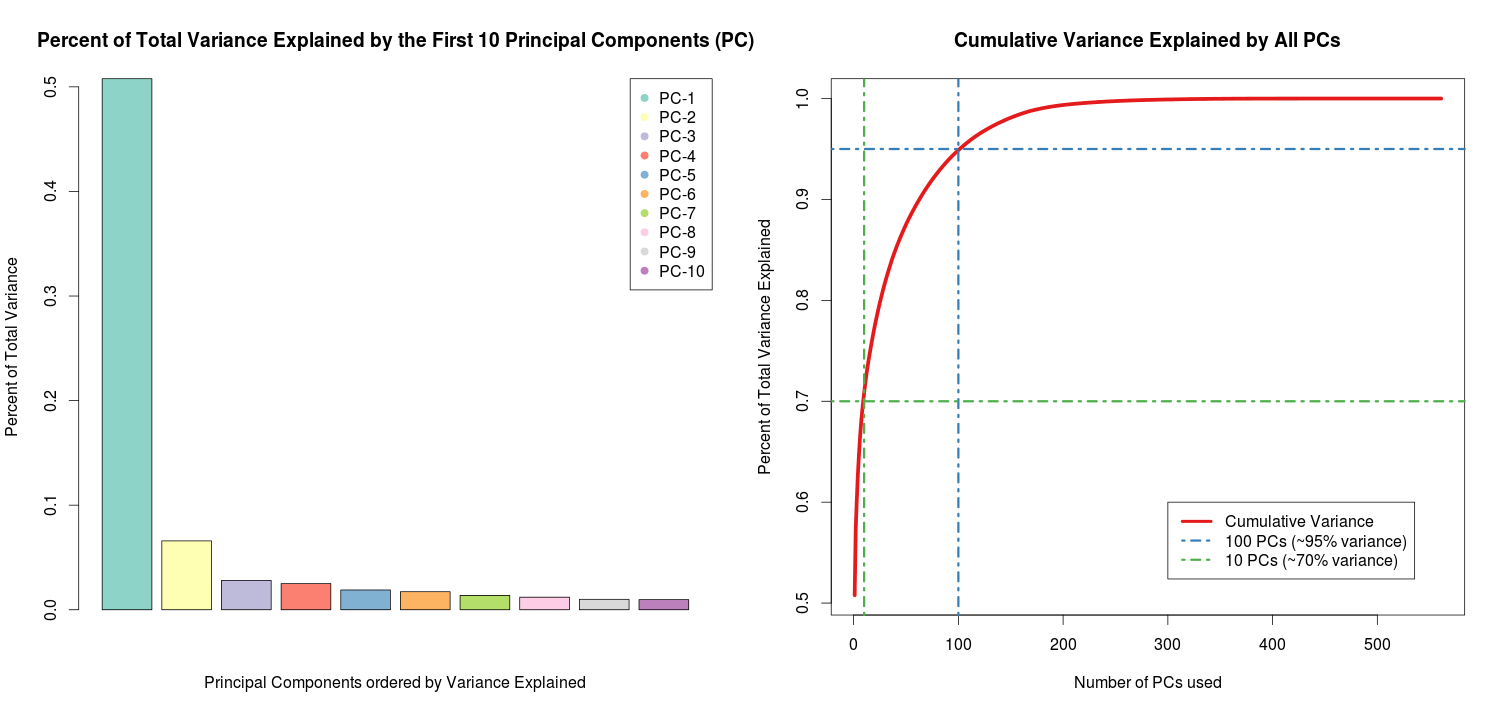
\includegraphics[width=\textwidth]{../figures/pca_v2}
  \label{fig:pca}
  \caption{ left) The variance capture by the top 10 PCs. right) Total
  variance as a function of number of PCs chosen. 1 PC, 10 PCs, and 100PCs capture $50\%$, $70\%$, and $95\%$ of the total variance 
  respectively.}
\end{figure}

\subsection{Baseline Model Performance}
The uniform random classifier had an average cross-validation (CV) error of $.831$, 
a test error of $.833$. Running 1000 iterations of bootstrapping with replacement:\\\\
\texttt{ sample\_data = sample(training\_data, size=nrow(training\_data)/2, replace=T) }
\\provides 1000 error rates that can be used to calculate average error and variance. 
For the base model, bootstrapping gives a mean, $\mu$ ,error of $.833$ and std. error,
$\sigma$, of $5.0\times10^{-3}$. The average confusion matrix, below, shows which activities were the hardest to classify. True values are rows and predicted values are columns.

\begin{center}
\begin{tabular}{l*{6}{c}r}
Activity              & laying & sitting & standing & walk & walkdown  & walkup \\
\hline
laying & 22.5  & 22.7  & 10.3  & 22.2  & 23.1  & 10.6 \\
sitting & 19.1  & 21.4  & 10.1  & 18.6  & 20.5  & 12.5 \\
standing & 22.9  & 20.9  & 10.7  & 21.8  & 20.0  & 12.8 \\
walk    & 19.7  & 20.2  & 9.8  & 20.8  & 19.3  & 9.9 \\
walkdown & 14.6  & 16.8  & 7.9  & 15.2  & 15.2 & 8.9 \\
walkup & 18.1  & 17.0 & 7.8  & 16.8  & 17.6 & 8.4 \\
\end{tabular}
\end{center}

For example, the first row shows the distribution of predicted activities for all
activities whose true value was \texttt{laying}. It is safe to say that this model is not good.


\subsection{Tree Model Performance}
The resulting classification tree that is built from a reduced training set with
10 variables has an average CV error of $.255$ and a test error of $.232$. Using the same
 bootstrap technique as previously we get $\mu = .255$ and $\sigma = 0.018$. The 
 average confusion matrix was:

\begin{center}
\begin{tabular}{l*{6}{c}r}
Activity              & laying & sitting & standing & walk & walkdown  & walkup \\
\hline
laying & 104.7 & 5.3 & 0.0 & 0.0 & 0.0 & 1.4 \\
sitting &  8.5 & 46.5 & 47.1 & 0.0 & 0.0 & 0.1 \\
standing &  0.0 & 17.1 & 92.0 & 0.0 & 0.0 & 0.0 \\
walk    &  0.0 & 0.0 & 0.0 & 79.5 & 4.6 & 15.6 \\
walkdown & 0.0 & 0.0 & 0.0 & 16.2 & 50.2 & 12.2 \\
walkup & 0.0 & 0.3 & 0.0 & 15.8 & 5.5 & 64.1 \\
\end{tabular}
\end{center}

The resulting classification tree that is built from a reduced training set with 100
variables has an average CV error of $.251$ and a test error of $.205$. Bootstrapping gives
us the following properties of the error: $\mu = .256 $ and $\sigma = .017$. The average confusion
matrix was:
\begin{center}
\begin{tabular}{l*{6}{c}r}
Activity & laying & sitting & standing & walk & walkdown  & walkup \\
\hline
laying & 105.2 & 4.8 & 0.0 & 0.0 & 0.0 & 1.4 \\
sitting &  8.9 & 46.8 & 46.4 & 0.0 & 0.0 & 0.1 \\
standing &  0.0 & 16.6 & 92.4 & 0.0 & 0.0 & 0.1\\
walk    &  0.0 & 0.0 & 0.0 & 82.5 & 4.1 & 13.1\\
walkdown &  0.0 & 0.0 & 0.0 & 16.8 & 49.3 & 12.5\\
walkup &  0.0 & 0.1 & 0.0 & 16.5 & 5.7 & 63.4\\
\end{tabular}
\end{center}

\section{Conclusion}
Both tree models are significantly better than the naive baseline model, however, the 
tree model that uses a 100-dimensional dataset that covers more variance did not perform
significantly better than the tree trained on a 10-dimensional dataset. This illustrates
the importance of dimensionality reduction when working with complex datasets. 
In addition, the confusion matrices show that my tree models have a difficult time
classifying between "sitting" and "standing" and does best identifying "laying".

\end{document}